\section{Show Case Examples}
Here we are going to introduce and show different tests we have done through the usage of the multiple instruments defined during the \autoref{sec:tools} chapter. We will proceed gradually, by giving first an example of how you can start minikube, then moving on showing the checks you can perform for testing everything is working correctly.
\subsection{Show case Minikube Project}
Now, we are going to see the basic procedures to start a cluster. After downloading and setting all the tools needed in \autoref{sec:tools}, we will open our terminal and start our minikube, composed of only one node (both master and worker). You'll see an image as shown in \autoref{fig:minikube start}. \\
Now, we'll proced to launch the following code, which it will configure a web application, composed of four pods. These pods will be launched inside the default namespace:
\begin{lstlisting}[language=yaml, caption={Deployment web application}, label={lst:yaml_4_pods}]
apiVersion: apps/v1
kind: Deployment
metadata:
  name: vite-deployment
  labels:
    app: vite
spec:
  replicas: 4
  selector:
    matchLabels:
      app: vite
  template:
    metadata:
      labels:
        app: vite
    spec:
      containers:
      - name: vite
        image: matteofrigo1618/vite_application:v1.0
        ports:
        - containerPort: 3000
\end{lstlisting}
Following, we will write the service yaml document. This code is useful to expose one or multiple pods to the external network of minikube, i.e. our local system. In addition, the service type will provide load balancing between all pods, managing the multiple requests from different users.

\begin{lstlisting}[language=yaml, caption={Service web application service}, label={lst:yaml_4_pods_svc}]
apiVersion: v1
kind: Service
metadata:
  name: webapp-service # Name we want to assign the service
spec:
  type: NodePort # It's the type of port required to connect with the external
  selector:
    app: vite # we define at which pods it needs to connect to 
  ports:
    - protocol: TCP
      port: 3000 # Internal exposed port inside cluster.
      targetPort: 3000 
      nodePort: 30100 # Port to extern cluster. Must be between 300000 - 32767.
\end{lstlisting}

Next, by sending the following commands in CLI you will create the four pods and a service which enable us to connect to it. \\
\begin{lstlisting}[ caption={Launch deployment and service}]
% For my project they were. Deployment:
kubectl apply -f vite_application.yaml
% Service:
kubectl apply -f vite-svc.yaml
\end{lstlisting}
Now, we have launched the two YAML documents, i.e. \hyperref[lst:yaml_4_pods_svc]{Service} and \hyperref[lst:yaml_4_pods]{Deployment}, to create and make our application available to external. If everything worked fined, by passing the command "kubectl get all", you should see the result in \autoref{fig:kubectl_get_all}.
\begin{figure}[h!]
    \centering
    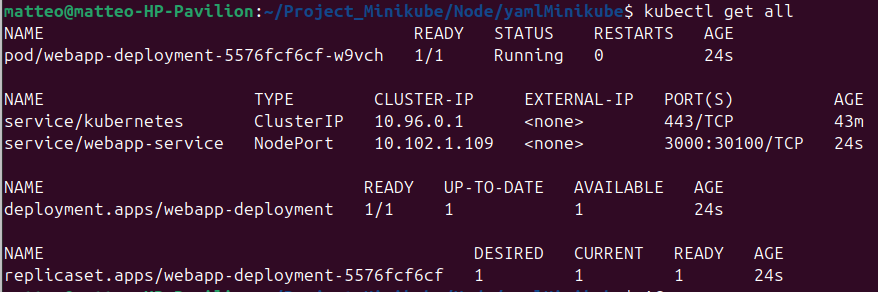
\includegraphics[width=0.65\textwidth]{images/kubectl_get_all.png}
    \caption{Minikube get all components}
    \label{fig:kubectl_get_all}
\end{figure} \\
To access the application we have created, we will use a tunnel to connect to Minikube. With the following command, you will be able to connect to the application:
\begin{lstlisting}[ caption={Open tunnel to minikube}]
$ minikube service webapp-service --url
http://<localhostIP>:<PortNumber Tunnel>
! Because you are using a Docker driver on linux, the terminal needs to be open to run it.
\end{lstlisting}
If you have run it, you will see that the "PortNumber Tunnel" isn't 30100 as specified before, but a random value generated by Minikube. This is because we are creating a tunnel from our local system, to the minikube cluster. This command is \textbf{necessary} for the connection because we are using minikube with driver of Docker. It would be different the procedures to connect to the web application if we were using VirtualBox or VM-based drivers.

\subsection{Show case Resource Quotas}
Here we are going to show an example of implementation of a ResourceQuota constraints across two namespaces, which logically divide a clusters, isolating the different resources. This can be seen as a perfect example of how we can differentiate our cloud resources among the customers, based on what contract we have with them.
\begin{lstlisting}[language=yaml, caption={Deployment namespace ResourceQuotas}, label={lst:resource_quota_deployment}]
apiVersion: v1
kind: ResourceQuota
metadata:
  name: quota-tenant-a
  namespace: tenant-a
spec:
  hard:
    # Minimum amount of resources they will have
    requests.cpu: "2"
    requests.memory: 4Gi
    # Maximum amount of resources they can take
    pods: "4"
    limits.cpu: "8"
    limits.memory: 10Gi
---
apiVersion: v1
kind: ResourceQuota
metadata:
  name: quota-tenant-b
  namespace: tenant-b
spec:
  hard:
    # Minimum amount of resources they will have
    requests.cpu: "1"
    requests.memory: 10Mi
    # Maximum amount of resources they can take
    pods: "4"
    limits.cpu: "2"
    limits.memory: 50Mi
\end{lstlisting}
We apply the constraint to the two namespaces and then to the cluster. Remember, that first we need to create the two namespaces if you haven't already done it:
\begin{lstlisting}[ caption={Apply Resource Quota feature}, label={listing:create-namespace}]
$ kubectl create namespace tenant-a
$ kubectl create namespace tenant-b
$ kubectl apply -f resource_quota_exceed_mem.yaml
\end{lstlisting}
As we can see for tenant-b, we allocated 50MB of memory as limit. Now, we want to purposly use more of that, to show what it's going to happen when we try to use more memory than we should. We want to test it because it can happen that a group team has certain limit of resources, but the \textbf{application requires} more of that. So we should block them and  change contract or give more resources based on the relationship we have with the client, for example if we are in a company environment between departments. Here's the python code we will use to trigger this limit:
\begin{lstlisting}[language=Python, caption={LimitRange Setup}]
import time
def allocate_memory(mb):
    size = mb*1024*1024
    return bytearray(size)

time.sleep(5)
print("We start by allocating 10 MB of memory")
mem_chunks = [allocate_memory(10)]  # 10 MB
time.sleep(30)

print("After ten seconds we will try allocating 50MB")
try:
    mem_chunks.append(allocate_memory(50))  # Supera i 50 MB totali
    print("Process still alive")
except MemoryError:
    print(" MemoryError: we overflow the limit")
    
# Wait to observe the pod behaviour
time.sleep(60)
print("Finished")
\end{lstlisting}
After writing the code and creating the appropriate Docker image of the program, we shall configure the deployment. We can reuse the code of \autoref{lst:yaml_default}, but modifying the following lines:
\begin{lstlisting}[language=yaml, caption={Deployment exceeding memory application}]
*** Configuration Listing 2 ***
  namespace:tenant-b
  labels:
    app: exceed_memory
spec:
  replicas: 1               # Number of pods to generate
  *** Configuration Listing 2 ***
      containers:
        image: <you-image-name-python>
        resources:
          requests:
            cpu: "500m" 
            memory: "5Mi" 
          limits:
            cpu: "1"
            memory: "50Mi"
\end{lstlisting}
Obviously, if we try to configure more resources instead of the limit of what we configured in the ResourceQuota, the deployment will fail, without launching the requested pod and forcing us to configure the pod in a more coeherent way. You can see a scenario of this problem in \autoref{subsub:possible errors}. After applying the \hyperref[lst:yaml_default]{deployment} we can see the logs of the application by launching:
\begin{lstlisting}[ caption={Logs Pod}]
$ kubectl get pods -n tenant-b
% Get the name of the pod to be used next:
$ kubectl logs <name-pod> -n tenant-b
\end{lstlisting}
What it's going to happen is figured in \autoref{fig:kubectl_OOMKilled}. Where we can see the looping of three status for the specific pod:
\begin{itemize}
    \item Running. Pod is running as it should be. It's before we try to configure more than the limit of memory for the pod.
    \item OOMKilled. The pod has gone over the limit of memory we set. The status tells that kubernetes killed that process and reload it from beginning. 
    \item CrashLoopBackOff. The pod continually crash and kuberentes is waiting some time before restarting it.
\end{itemize}
\begin{figure}[h!]
    \centering
    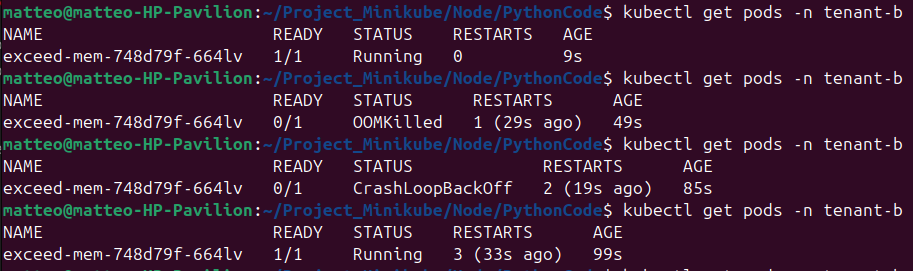
\includegraphics[width=0.7\textwidth]{images/OOMKilled_exceed_memory.png}
    \caption{Pod exceeding memory}
    \label{fig:kubectl_OOMKilled}
\end{figure} 
\subsubsection{Addional constrainments}
In addition to the constraints of the ResourceQuota. We can configure a namespace quotas with different classes of priority and resource quantity. In fact, based on the pod we launch, we can define different constraints inside the same namespace:
\begin{lstlisting}[language=yaml, caption={Class ResourceQuota setup}]
apiVersion: v1
kind: List
items:
- apiVersion: v1
  kind: ResourceQuota
  metadata:
    name: pod-high
    namespace: <namespace name>
  spec:
    hard:
      cpu: "6"
      memory: "16Gi"
      pods: "6"
    scopeSelector:
      matchExpressions:
      - operator: In
        scopeName: PriorityClass
        values: ["high"]

- apiVersion: v1
  kind: ResourceQuota
  metadata:
    name: pod-low
    namespace: <namespace name>
  spec:
    hard:
      cpu: "2"
      memory: "4Gi"
      pods: "2"
    scopeSelector:
      matchExpressions:
      - operator: In
        scopeName: PriorityClass
        values: ["low"]
\end{lstlisting}
Then, in the deployment of the pods, we can add our additional class constraint:
\begin{lstlisting}[language=yaml, caption={Set class - deployment}]
 *** Deployment configurations ***
 resources:
      requests:
        memory: "10Gi"
        cpu: "500m"
      limits:
        memory: "10Gi"
        cpu: "500m"
  priorityClassName: high # Value defined in the matchExpression.values
\end{lstlisting}
Obviously, we have just scratch the surface of additional constraints we can set to the ResourceQuota.

\subsection{Show case combination ResourceQuotas and LimitRanges}
Until now we have explore the ResourceQuota setting and what to insert inside the deployment of your containers. What if the team managing it, forgets to configure the limit and request values inside the deployment? What we can do is to combine LimitRange and ResourceQuota:
\begin{lstlisting}[language=yaml, caption={LimitRange setup with ResourceQuota}, label={lst:ResourceQuota_and_LimitRange}]
apiVersion: v1
kind: LimitRange
metadata:
  name: limit-range-constraints
  namespace: tenant-b
spec:
  limits: # We need to respect constraint of ResourceQuotas of before
  - default: 
      cpu: 1000m
      memory: 50Mi
    defaultRequest: 
      cpu: 500m
      memory: 5Mi
    type: Container
\end{lstlisting}
With the code of \autoref{lst:ResourceQuota_and_LimitRange}, we consider it with the implementation of ResourceQuota of \autoref{lst:resource_quota_deployment}, where we set default limits and request for all the pods inside a namespace. So, when deploying our application \autoref{lst:yaml_default}, if we want we can remove the "resources" fields and launch it inside the namespace, since its set automatically by the limitRange. With this method, if a developer forget to set the resources used by the application, or for standardizing deployment, we can initialized them by default. In fact, after deploying any application deployment you will see the default request and limit constraints by sending the following line:
\begin{lstlisting}[caption={Show constraints deployment}]
$ kubectl describe quota -n <namespace> 
$ kubectl describe limitrange -n <namespace> 
\end{lstlisting}

\subsection{Show case Access Control}
Another measure we can apply to our cluster is access control and network policies, which we saw in \autoref{subsec:access control} and \autoref{subsec:network policies}. These functionalities let us impose strict rules inside our namespace for every tenant. We divide the two into:
\begin{itemize}
    \item Network policies, as we also saw before in \autoref{subsec:network policies}, we defined a general rule where different pods inside a namespaces, cannot communicate with others, so isolating the network connections between namespaces. Here we are not going to implement it, since it's personal for specific cluster and the implementation of it is generally equal to any other definition of service or resources inside kubernetes.
    \item Role-based access control, where we impose rule the services apply. This can change based on what activity or access we want to give to the pods owned by a specific tenant. In \autoref{subsub:role-based access control} we described an example of only observation role for the customer, making the administrator of the cluster the only one who can change the characteristics or setting of a namespace. This is a feature we can implement, in addition to many other based on the service, security and management we want to give to the customers. \textbf{By default}, the pods or containers cannot access any information related to the cluster, so implementing these rules let a tenant access additional resources about the cluster (based on what we permit it to do).
\end{itemize}

\subsubsection{Role‑Based Access Control}
\label{subsub:role-based access control}
Below we implement the yaml code needed to create, manage and bind a rule to the service account. First lets create the namespace where a customer tenant can work, through the command \autoref{listing:create-namespace} with name "torino-tenant". Next, we create and apply the following code through the "kubectl apply" command:
\begin{lstlisting}[language=yaml, caption={ServiceAccount, rule and ruleBinding}, label={lst:SerAcc-rule-binding}]
# we define a Service account
apiVersion: v1
kind: ServiceAccount
metadata:
  name: service-torino
  namespace: torino-tenant
---
# we define a Role we want to apply to our service account
apiVersion: rbac.authorization.k8s.io/v1
kind: Role
metadata:
  name: read-pod
  namespace: torino-tenant
rules:
- apiGroups: [""]
  resources: ["pods"]
  verbs: ["get", "list"]
---
# we define the bind between role and service account
apiVersion: rbac.authorization.k8s.io/v1
kind: RoleBinding
metadata:
  name: bind-torino
  namespace: torino-tenant
subjects:
- kind: ServiceAccount
  name: service-torino
  namespace: torino-tenant
roleRef:
  kind: Role
  name: read-pod
  apiGroup: rbac.authorization.k8s.io
\end{lstlisting}
After creating the service account, role and bind these two together. We can implement the service account related to pod resources inside the namespace. In fact, what I image from my example is to create a pod resource which was able to access and look at the pods details of his own namespace. Below we can see the code used to achieve and create this pod. We used bitnami, which it's used to execute kubectl commands inside a pod, mainly used for debugging purposes.
\begin{lstlisting}[language=yaml, caption={Lauch pod with specific ServiceAccount}, label={lst:serviceAccount-pod}]
apiVersion: v1
kind: Pod
metadata:
  name: pod-reader
  namespace: tenant-b
spec:
  serviceAccountName: pod-reader
  containers:
  - name: reader
    image: bitnami/kubectl:latest
    command: ["sleep", "3600"] # Used to keep the container alive
\end{lstlisting}
Then, after applying the specified code, we can see the result by writing the following code in the cmd: 
\begin{lstlisting}[caption={Show constraints deployment}]
$ kubectl exec -n torino-tenant -it pod-reader -- sh
# -- Enter pod ssh --
$ kubectl get pods
$ kubectl get pods -o wide
$ kubectl get deployments
\end{lstlisting}
The result of the previous commands will be the possibility to access only the pods information. In fact, we can see the result also in the following image:
\begin{figure}[h!]
    \centering
    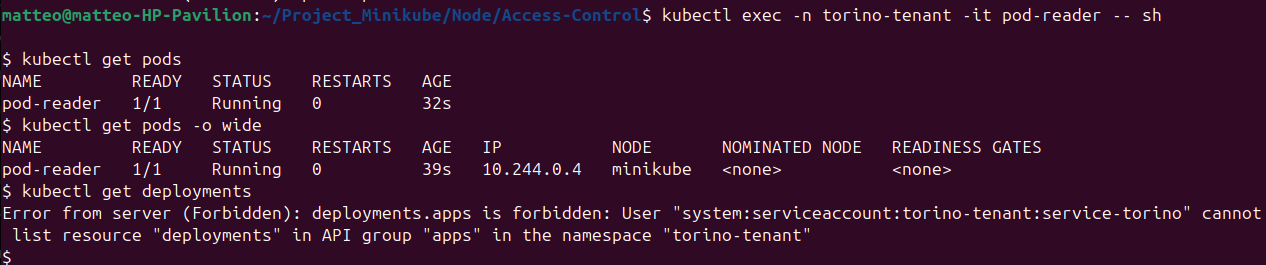
\includegraphics[width=0.8\textwidth]{images/kubectl-pod.png}
    \caption{Retrieve information from inside pod}
    \label{fig:kubectl-pod}
\end{figure} \\